%%===========================================================%%
%%                                                           %%
%%                     DE/DX ADJUSTMENT                      %%
%%                                                           %%
%%===========================================================%%


\chapter{\texorpdfstring{d$\bm{E}$/d$\bm{x}$}{dE/dx} adjustment}\label{chap:dEdxCorrection}

Particle identification in our analyses is done using merged information from the TPC (specific energy loss of tracks $dE/dx$) and from the TOF (time of hit macthed to TPC track). As can be seen in Fig.~\ref{fig:dEdxDataVsMC}, $dE/dx$ information from the MC events simulated in STARsim (in red) poorely matches the data points (black). This results e.g. in large systematic error of estimate of particle identification efficiency.

This problem was discussed under ticket \#3272~(Ref.~\cite{dedxTicket}). There were trials to improve the TPC calibration in simulation, but the problem remained. It was finally concluded that the origin of the problem lies in the model of energy loss used in the STARsim, therefore any further action was postponed. 

In order to tune simulated reposponse of the TPC in terms of $dE/dx$, hence also reduce the systematic uncertainty related to particle identification, a correction method was developed based on proper transformation (recalculation) of simulated $dE/dx$ to obtain new $dE/dx$ whose distribution matches the data.
% It is possible to transform dE/dx in MC to make it follow the shape of dE/dx in the data. 
We know that $n^{\sigma}_{X}$ (where $X=\pi, K, p$, ...) variable for particle $X$ follows a gaussian distribution
\begin{equation}n^{\sigma}_{X} = \Big( \ln{\frac{dE/dx}{\langle dE/dx\rangle_{X}}} \Big) / \sigma_{dE/dx},~~~~~f(n^{\sigma}_{X}) = \mathcal{N}(n^{\sigma}_{X}; \mu=0,\sigma=1),\end{equation}
therefore $dE/dx$ itself by definition follows log-normal distribution:
\begin{equation}f(dE/dx) = \mathcal{L}og\mathcal{N}(dE/dx; \mu=\langle dE/dx\rangle,\sigma=\sigma_{dE/dx}) = \frac{1}{\sqrt{2\pi}\cdot \sigma\cdot dE/dx}e^{-\frac{\ln^{2}{\frac{dE/dx}{\langle dE/dx\rangle}}}{2\sigma^{2}}}.\end{equation}
The desired transformation should preserve the shape of $dE/dx$ distribution so that it is still described by $\mathcal{L}og\mathcal{N}$, however it should change $\mu$ and $\sigma$ so that these values are euqal to ones in the data. The transformation that satisfies above postulate is
\begin{equation}dE/dx' = c\cdot (dE/dx)^{a}.\label{eq:dedxTranformation}\end{equation}
Parameters of the distribution $\mathcal{L}og\mathcal{N}(dE/dx')$ are then
\begin{equation}\mu' = c\cdot\mu^{a},~~~~\sigma' = a\cdot\sigma.\end{equation}
From above we get formulae for parameters of the transformation:
\begin{equation}a=\sigma'/\sigma,~~~~c = \frac{\mu'}{\mu^{a}}.\label{eq:dedxPatameters}\end{equation}%
%
To sum up, one has to find the MPV and width parameter of the $dE/dx$ spectrum of each particle in the data and MC, and use relations \eqref{eq:dedxPatameters} in order to find parameters of the transformation introduced in Eq.~\eqref{eq:dedxTranformation}.

The most challenging part of the task was extraction of the $\langle dE/dx\rangle$ and $\sigma_{dE/dx}$ from the data. In case of MC one can select tracks matched to true-level particles of given ID and thus separate $dE/dx$ of different particles, which makes extraction of the distribution shape straightforward. Unfortunately, it is not possible to apply the same method to the data - here one has to deal with overlapping of the reconstructed $dE/dx$ from different particles. Therefore fits of sum of $f(dE/dx)$ corresponding to different particles were performed to reconstructed track $dE/dx$ in narrow momentum bins. The width of momentum bins was chosen to compromize statistics and validity of assumption of constant parameters of $dE/dx$ distribution over bin range.

It was found during the fitting that log-normal distribution is not a perfect model of the reconstructed $dE/dx$. The problems with description of the data were mainly in the tail-part of the distribution from single particle. Precise model was necessary to obtain satistactory quality of fits and trustworthy values of parameters. After some reasearch the best model of $dE/dx$ distribution from single particle was found to be%  Eq.~\eqref{eq:expTail}:%
%
\begin{equation}\label{eq:expTail}
	f(dE/dx)=\left\{
                \begin{array}{ll}
                  \frac{A}{\sqrt{2\pi}\cdot \sigma\cdot dE/dx}\exp{\Bigg(-\frac{1}{2}\Big(\frac{\ln{\frac{dE/dx}{\langle dE/dx\rangle}}}{\sigma}\Big)^{2}\Bigg)} & \textrm{for}~\frac{\ln{\frac{dE/dx}{\langle dE/dx\rangle}}}{\sigma} \leq k \\
                  \frac{A}{\sqrt{2\pi}\cdot \sigma\cdot dE/dx}\exp{\Bigg(-k\cdot \frac{\ln{\frac{dE/dx}{\langle dE/dx\rangle}}}{\sigma} + \frac{1}{2}k^{2} \Bigg)} & \textrm{for}~\frac{\ln{\frac{dE/dx}{\langle dE/dx\rangle}}}{\sigma} > k.
                \end{array}
              \right.
\end{equation}%
%
Such form was motivated by the function presented in Ref.~\cite{AlternativeToCrystallBall}, here adopted for the log-normal instead of normal distribution. Because the modification of the log-normal distribution is introduced only at high-end tail, the validity of the transformation discussed above still holds. To reduce fit complexity the $k$ parameter was set the same for all particle species and fixed  to value equal $2.2$, which worked well for both data and embedded MC. Particles and their anti-particles were assumed to have the same $dE/dx$ distributions for a given momentum and were analyzed together. The sample fit in a single momentum bin can be found in Fig.~\ref{fig:dEdxFit}. Fits in all momentum bins can be found in Appendix~\ref{appendix:dEdxAdjustment}.
%
%
%---------------------------
\begin{figure}[ht!]%
\centering%
\includegraphics[width=\linewidth,page=12]{graphics/dedx/dEdx_fitPerMomentumBin_4thIteration.pdf}\vspace{-5pt}%
\caption[Sample fit to dE/dx spectrum in the data in single momentum bin.]%
{Sample fit of sum of functions from Eq.~\eqref{eq:expTail} corresponding to different particle species to dE/dx spectra in the data in a single momentum bin.}\label{fig:dEdxFit}\vspace{10pt}
\end{figure}
%---------------------------
%
%
%---------------------------
\begin{figure}[hb!]\vspace{-45pt}
\centering
\parbox{0.4725\textwidth}{
  \centering
  \begin{subfigure}[b]{\linewidth}{
                \subcaptionbox{\label{fig:dEdxMeanOffsetMC}}{\includegraphics[width=\linewidth]{graphics/dedx/dEdxMeanOffset_allPIDs.pdf}\vspace*{-10pt}}}
  \end{subfigure}\\[-3pt]
  \begin{subfigure}[b]{\linewidth}\addtocounter{subfigure}{1}{
                \subcaptionbox{\label{fig:dEdxMeanOffsetData}}{\includegraphics[width=\linewidth]{graphics/dedx/dEdxMeanOffset_allPIDs_data.pdf}\vspace*{-10pt}}}
  \end{subfigure}
}
\quad
\parbox{0.4725\textwidth}{
  \centering
  \begin{subfigure}[b]{\linewidth}\addtocounter{subfigure}{-2}{
                \subcaptionbox{\label{fig:dEdxWidthMC}}{\includegraphics[width=\linewidth]{graphics/dedx/dEdxWidth_allPIDs.pdf}\vspace*{-10pt}}}
  \end{subfigure}\\[-3pt]
  \begin{subfigure}[b]{\linewidth}\addtocounter{subfigure}{1}{
                \subcaptionbox{\label{fig:dEdxWidthData}}{\includegraphics[width=\linewidth]{graphics/dedx/dEdxWidth_allPIDs_data.pdf}\vspace*{-10pt}}}
  \end{subfigure}
}\vspace{-5pt}%
\caption[Parameters of reconstructed track dE/dx as a function of reconstructed momentum for a few particle species.]{Difference between MPV of dE/dx predicted by Bichsel parametrization and obtained from the fit of Eq.~\eqref{eq:expTail} to dE/dx distribution in the data (\ref{fig:dEdxMeanOffsetData}) and MC sample (\ref{fig:dEdxMeanOffsetMC}) and dE/dx width parameter in data (\ref{fig:dEdxWidthData}) and MC (\ref{fig:dEdxWidthMC}) as a function of reconstructed particle momentum for a few particle species. Solid lines represent fits to points of corresponding color. Only statistical errors are shown.}\label{fig:dEdxParametersMC}
\end{figure}
%---------------------------


Results of the fits for all considered particle species (pions, kaons, protons, electrons and deuterons) are commonly presented in Fig.~\ref{fig:dEdxParametersMC} with color markers. Figures \ref{fig:dEdxMeanOffsetData} and~\ref{fig:dEdxMeanOffsetMC} show the offset of the MPV of reconstructed $dE/dx$ relative to the Bichsel parametrization in the data and embedded MC, respectively, and Fig.~\ref{fig:dEdxWidthData} and~\ref{fig:dEdxWidthMC} show the width of reconstructed $dE/dx$ (in the same order). Function able to qualitatively describe dependence of the parameters as a function of track momentum was empirically found to be given by Eq.~\eqref{eq:dEdxParametrization}:
%
\begin{equation}\label{eq:dEdxParametrization}
	g(p) = P_{1} + P_{2}\cdot \exp{\left(-P_{3}\cdot p\right)} + P_{4}\cdot \arctan{\big(P_{5}\cdot(p-P_{6})\big)}
\end{equation}
%
This function was fitted to points corresponding to each particle type and fit result is shown in Fig.~\ref{fig:dEdxParametersMC} with lines colored in accordance to markers. Values of parameters of above function are tabulated in Tab.~\ref{tab:dEdxParametersMC}.

\begin{table}[hb!]\vspace{5pt}\centering%
\subcaptionbox{\label{tab:dEdxParametersMC}}{\centering%
 \begin{tabular}{r||c|c|c|c|c|c||c|c|c|c|c|c}%\hline
 \multirow{2}{*}{\textbf{PID}} &  \multicolumn{6}{c||}{\bm{$\langle dE/dx\rangle_{\textrm{\textbf{Bichsel}}} - \langle dE/dx\rangle_{\textrm{\textbf{MC}}}$}} & \multicolumn{6}{c}{\bm{$\sigma(dE/dx)_{\textrm{\textbf{MC}}}$}} \\ \cline{2-13}%
  & $P_{1}$ & $P_{2}$ & $P_{3}$ & $P_{4}$ & $P_{5}$ & $P_{6}$ & $P_{1}$ & $P_{2}$ & $P_{3}$ & $P_{4}$ & $P_{5}$ & $P_{6}$ \\ \Xhline{2\arrayrulewidth}
$\bm{\pi^{\pm}}$ &\scriptsize 7.183e-8 &\scriptsize -1.647e-4 &\scriptsize 41.68 &\scriptsize          &\scriptsize         &\scriptsize          &\scriptsize 0.0705 &\scriptsize      &\scriptsize      &\scriptsize -1.42e-3 &\scriptsize 9.860 &\scriptsize 0.951 \\ \hline
$\bm{K^{\pm}}$ &\scriptsize 4.359e-8 &\scriptsize -9.285e-6 &\scriptsize 7.697 &\scriptsize          &\scriptsize         &\scriptsize         &\scriptsize 0.0511 &\scriptsize 0.034 &\scriptsize 1.675 &\scriptsize 1.01e-2 &\scriptsize 4.934 &\scriptsize 0.528 \\ \hline
$\bm{p,\bar{p}}$ &\scriptsize 3.556e-8 &\scriptsize -8.621e-6 &\scriptsize 3.980 &\scriptsize          &\scriptsize         &\scriptsize         &\scriptsize 0.0630 &\scriptsize -7.725 &\scriptsize 27.17 &\scriptsize 3.37e-3 &\scriptsize 5.245 &\scriptsize 0.670 \\ \hline
$\bm{e^{\pm}}$ &\scriptsize -6.219e-8 &\scriptsize 2.065e-7 &\scriptsize 3.241 &\scriptsize          &\scriptsize         &\scriptsize           &\scriptsize 0.0354 &\scriptsize 0.982 &\scriptsize 26.58 &\scriptsize 1.79e-2 &\scriptsize 41.515 &\scriptsize 0.095 \\ \hline
$\bm{d,\bar{d}}$ &\scriptsize -1.305e-6 &\scriptsize -5.268e-6 &\scriptsize 3.486 &\scriptsize ~~~~~~~~~~~ &\scriptsize ~~~~~~~ &\scriptsize ~~~~~~ &\scriptsize 0.0967 &\scriptsize -1526 &\scriptsize 18.75 &\scriptsize          &\scriptsize         &\scriptsize         
\end{tabular}%
}\\ \centering%
\subcaptionbox{\label{tab:dEdxParametersData}}{%
\begin{tabular}{r||c|c|c|c|c|c||c|c|c|c|c|c}%\hline
 \multirow{2}{*}{\textbf{PID}} &  \multicolumn{6}{c||}{\bm{$\langle dE/dx\rangle_{\textrm{\textbf{Bichsel}}} - \langle dE/dx\rangle_{\textrm{\textbf{Data}}}$}} & \multicolumn{6}{c}{\bm{$\sigma(dE/dx)_{\textrm{\textbf{Data}}}$}} \\ \cline{2-13}
  & $P_{1}$ & $P_{2}$ & $P_{3}$ & $P_{4}$ & $P_{5}$ & $P_{6}$ & $P_{1}$ & $P_{2}$ & $P_{3}$ & $P_{4}$ & $P_{5}$ & $P_{6}$ \\ \Xhline{2\arrayrulewidth}
 $\bm{\pi^{\pm}}$ & \scriptsize -1.399e-8 & \scriptsize 2.012e-7 & \scriptsize10.39 & \scriptsize&             \scriptsize&                \scriptsize&         \scriptsize 0.0734 & \scriptsize1.907 & \scriptsize31.86 & \scriptsize-8.20e-4 & \scriptsize 22.788 & \scriptsize 0.653\\ \hline
 $\bm{K^{\pm}}$ & \scriptsize    2.325e-9 & \scriptsize -3.690e-6 & \scriptsize 8.712 & \scriptsize&           \scriptsize&               \scriptsize&          \scriptsize 0.0808 &  \scriptsize -0.040 & \scriptsize7.951 & \scriptsize 5.62e-3 & \scriptsize -17.08 &  \scriptsize 0.269\\ \hline
 $\bm{p,\bar{p}}$ & \scriptsize -1.458e-7 & \scriptsize 0.6655 &   \scriptsize59.06 & \scriptsize 1.171e-7 &    \scriptsize 4.660 &       \scriptsize 0.644 &   \scriptsize0.0795 & \scriptsize 0.181 & \scriptsize12.12 & \scriptsize& \scriptsize& \scriptsize\\ \hline
 $\bm{e^{\pm}}$ & \scriptsize   9.005e-8 &  \scriptsize 2.494e-7 & \scriptsize 8.834 & \scriptsize&              \scriptsize&              \scriptsize&          \scriptsize 0.0680 & \scriptsize 8.8e-4 & \scriptsize 1.549 & \scriptsize& \scriptsize& \scriptsize\\ \hline
 $\bm{d,\bar{d}}$ & \scriptsize -1.910e-7 & \scriptsize 5.637e-3 &  \scriptsize 14.48 & \scriptsize&               \scriptsize&              \scriptsize&          \scriptsize 0.1161 & \scriptsize -0.147 & \scriptsize 2.890 & \scriptsize& \scriptsize& \scriptsize%\\ \hline
\end{tabular}%
}\vspace{-7pt}\caption[Parameters of functions from Fig.~\ref{fig:dEdxParametersMC} describing reconstructed track dE/dx as a function of reconstructed momentum for a few particle species (STARsim MC).]{Parameters of functions from Fig.~\ref{fig:dEdxParametersMC} describing reconstructed track dE/dx as a function of reconstructed momentum for a few particle species. Blank cells denote parameters equal 0. Units of parameters $P_{i}$ are such that if one provides momentum in Eq.~\eqref{eq:dEdxParametrization} in GeV/$c$ the resultant offset of dE/dx MPV with respect to Bichsel parametrization is in GeV/cm, and the resultant $\sigma$ parameter is unitless.}\label{tab:dEdxParameters}
\end{table}%
%
%
%---------------------------
\begin{figure}[hb!]\vspace{-5pt}%
\centering%
\includegraphics[width=\linewidth,page=13]{graphics/dedx/dEdx_DataVsMC.pdf}\vspace{-5pt}%
\caption[Sample comparison of dE/dx spectrum between data and embedded MC in single momentum bin.]{Sample comparison of dE/dx spectrum between data and embedded MC (before and after $dE/dx$ adjustment) in a single momentum bin. Lower pad shows the ratio between embedded MC and data before and after $dE/dx$ adjustment. In both upper and lower padt the same color code is used. Only statistical errors are shown.}\label{fig:dEdxDataVsMCSingleBin}
\end{figure}
%---------------------------
%
The correctness of the entire procedure described in this section was verified by comparing the reconstructed track $dE/dx$ between the data and embedded MC without and with the $dE/dx$ transformed using Eq.~\eqref{eq:dedxTranformation} and parameters from Tab.~\ref{tab:dEdxParameters}. Some difficulty arised in this comparison due to inconsistent relative content of different particle species in the data and embedded MC sample. Problem was ressolved by separating $dE/dx$ histograms of different particle species (in the same way as it was done for extraction of $dE/dx$ MPV and $\sigma$ for each particle ID) and fitting the sum of histograms from different particle types to the data histogram (in momentum bins). The only free parameters in the fit were relative contents of histogram from singe particle type to the data histogram. A sample comparison between the $dE/dx$ in data and embedded MC is presented in Fig.~\ref{fig:dEdxDataVsMCSingleBin}. Comparison in all other momentum bins is contained in Appendix~\ref{appendix:dEdxAdjustment} (Fig.~\ref{fig:dEdxDataVsMC}). Fits were done for adjusted $dE/dx$ (filled green). Histograms for unadjusted $dE/dx$ (hashed red) were composed using the same relative content of particles as obtained from the fit of adjusted $dE/dx$. The ratio of the MC to the data shown in the lower pad of Fig.~\ref{fig:dEdxDataVsMCSingleBin} and Fig.~\ref{fig:dEdxDataVsMC} clearly demonstrates better agreement of the MC and the data after the adjustent in terms of position and width of peaks in $dE/dx$ spectrum.